\chapter{总体概述}

\section{软件概述}
\subsection{项目介绍}
随着计算机科学突飞猛进的发展,有越来越多的场合需要用到计算机进行科学计算、数据统计与数学模型的搭建。这些问题到最后都可归结于计算问题,因而一个优秀的计算器也是计算机中必备的软件,本项目也应运而生。

一般的计算器软件很难满足日渐增长的计算需求,亟需设计新型的计算软件,可以完成各种高级计算任务,满足多种人群的需要。

本项目将在Windows 10/MacOS/Linux操作系统环境下,以Python作为开发工具,实现一个兼备基本数学运算(四则运算与乘方),函数绘图,求排列组合、初等函数等常用数学工具以及诸如微分、积分等高级数学工具的多功能计算器。\\


\subsection{产品环境介绍}

本产品是一个多功能计算器。


如图2.1所示,我们的计算器的运行方式可以表示为如下流程:

1.通过多种途径接收用户的合理输入;

2.根据用户需求,计算相应的表达式并给出输出;

3.对于有错误的输入,尽可能给出错误信息,引导用户正确使用。

\begin{figure}[ht]
\centering
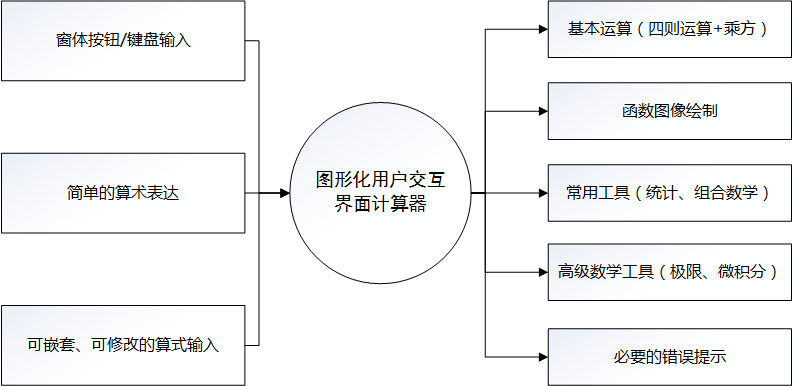
\includegraphics[width=9cm]{overview_1.png}
\caption{计算器输入输出概念图} \label{fig:overall_conception}
\end{figure}

本项目将使用Python 3.6的开发环境编写图形界面交互式计算器。


\section{软件功能}

本项目将在以下方面实现多功能计算:

1.四则运算+乘方(注意到乘方运算包含了开方运算)

2.函数图像的绘制

3.初等函数(三角函数、反三角函数、对数函数、指数函数)的运算

4.进制转换

5.阶乘、统计量、排列与组合的运算

6.矩阵的有关计算

7.极限、微分与积分的计算

8.常微分方程、FFT的计算\\

\section{用户特征}

本项目面向熟悉计算器的基本操作,且对数理统计、高等数学、科学计算与进制转换等方面有需求的全体人员。

如:

\quad 工程师

\quad 科研工作者

\quad 理工科学生

\quad 计算机从业者

\quad 统计工作者

\quad .....



\section{假设和依赖关系}

我们假设用户对计算器的运算规则有所了解,且会简单的计算机操作知识, 知晓数学操作的意义。

\section{开发期限}

本系统开发期限为一周。\\

